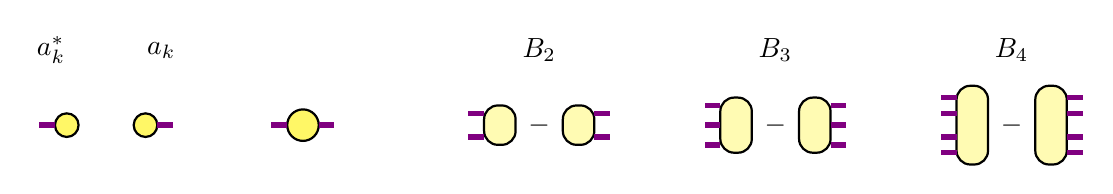
\begin{tikzpicture}


%vertex for $ a_k^* $
\filldraw[fill = yellow!60!white, thick] (0,0.25) circle (0.15);
\draw[line width = 2, red!50!blue] (-0.15,0.25) -- ++(-0.2,0);
\node at (-0.2,1.2) {$ a_k^* $};

%vertex for $ a_k $
\filldraw[fill = yellow!60!white, thick] (1,0.25) circle (0.15);
\draw[line width = 2, red!50!blue] (1.15,0.25) -- ++(0.2,0);  
\node at (1.2,1.2) {$ a_k $};

%vertex for $ \cN $
\filldraw[fill = yellow!60!white, thick] (3,0.25) circle (0.2);
\draw[line width = 2, red!50!blue] (2.8,0.25) -- ++(-0.2,0);
\draw[line width = 2, red!50!blue] (3.2,0.25) -- ++(0.2,0);  
\node at (3,1.2) {$ \cN $};


%vertex for $ B_2 $
\filldraw[thick, rounded corners = 5, fill = yellow!30!white] (5.3,0) rectangle ++(0.4,0.5);
\draw[line width = 2, red!50!blue] (5.3,0.1) -- ++(-0.2,0);
\draw[line width = 2, red!50!blue] (5.3,0.4) -- ++(-0.2,0);
\node at (6,0.25) {$ - $};
\filldraw[thick, rounded corners = 5, fill = yellow!30!white] (6.3,0) rectangle ++(0.4,0.5);
\draw[line width = 2, red!50!blue] (6.7,0.1) -- ++(0.2,0);
\draw[line width = 2, red!50!blue] (6.7,0.4) -- ++(0.2,0);
\node at (6,1.2) {$ B_2 $};


%vertex for $ B_3 $
\filldraw[thick, rounded corners = 5, fill = yellow!30!white] (8.3,-0.1) rectangle ++(0.4,0.7);
\draw[line width = 2, red!50!blue] (8.3,0) -- ++(-0.2,0);
\draw[line width = 2, red!50!blue] (8.3,0.25) -- ++(-0.2,0);
\draw[line width = 2, red!50!blue] (8.3,0.5) -- ++(-0.2,0);
\node at (9,0.25) {$ - $};
\filldraw[thick, rounded corners = 5, fill = yellow!30!white] (9.3,-0.1) rectangle ++(0.4,0.7);
\draw[line width = 2, red!50!blue] (9.7,0) -- ++(0.2,0);
\draw[line width = 2, red!50!blue] (9.7,0.25) -- ++(0.2,0);
\draw[line width = 2, red!50!blue] (9.7,0.5) -- ++(0.2,0);
\node at (9,1.2) {$ B_3 $};


%vertex for $ B_4 $
\filldraw[thick, rounded corners = 5, fill = yellow!30!white] (11.3,-0.25) rectangle ++(0.4,1);
\draw[line width = 2, red!50!blue] (11.3,-0.1) -- ++(-0.2,0);
\draw[line width = 2, red!50!blue] (11.3,0.1) -- ++(-0.2,0);
\draw[line width = 2, red!50!blue] (11.3,0.4) -- ++(-0.2,0);
\draw[line width = 2, red!50!blue] (11.3,0.6) -- ++(-0.2,0);
\node at (12,0.25) {$ - $};
\filldraw[thick, rounded corners = 5, fill = yellow!30!white] (12.3,-0.25) rectangle ++(0.4,1);
\draw[line width = 2, red!50!blue] (12.7,-0.1) -- ++(0.2,0);
\draw[line width = 2, red!50!blue] (12.7,0.1) -- ++(0.2,0);
\draw[line width = 2, red!50!blue] (12.7,0.4) -- ++(0.2,0);
\draw[line width = 2, red!50!blue] (12.7,0.6) -- ++(0.2,0);
\node at (12,1.2) {$ B_4 $};

\end{tikzpicture}